\documentclass[12pt]{article}
\usepackage{graphicx}
\usepackage{amsmath}
\usepackage{amssymb}
\usepackage{hyperref}
\usepackage{float}
\usepackage{booktabs}
\usepackage{caption}
\usepackage{subcaption}
\usepackage{xcolor}
\usepackage{listings}
\usepackage{geometry}
\geometry{a4paper, margin=1in}

% Define code listing style
\definecolor{codegreen}{rgb}{0,0.6,0}
\definecolor{codegray}{rgb}{0.5,0.5,0.5}
\definecolor{codepurple}{rgb}{0.58,0,0.82}
\definecolor{backcolour}{rgb}{0.95,0.95,0.92}

\lstdefinestyle{mystyle}{
    backgroundcolor=\color{backcolour},   
    commentstyle=\color{codegreen},
    keywordstyle=\color{magenta},
    numberstyle=\tiny\color{codegray},
    stringstyle=\color{codepurple},
    basicstyle=\ttfamily\footnotesize,
    breakatwhitespace=false,
    breaklines=true,
    keepspaces=true,
    numbers=left,
    numbersep=5pt,
    showspaces=false,
    showstringspaces=false,
    showtabs=false,
    tabsize=2
}

\lstset{style=mystyle}

\title{Assignment 3: Feedforward Neural Networks using PyTorch}
\author{Your Name and Student ID \\ Partner's Name and Student ID}
\date{\today}

\begin{document}

\maketitle

\section{Introduction}

This report presents our implementation and analysis of feedforward neural networks for digit classification using the MNIST dataset. We performed various experiments to explore hyperparameter selection, validation strategies, and feature visualization techniques.

\section{Task 1: MNIST Classification}

In this task, we implemented a basic two-layer fully connected neural network for classifying MNIST digits. The network architecture consists of an input layer (784 neurons), a hidden layer, and an output layer (10 neurons).

\subsection{Implementation Details}
Our implementation includes:
\begin{itemize}
    \item Loading and preprocessing the MNIST train and test datasets
    \item Implementing a two-layer neural network model
    \item Training using cross-entropy loss and Adam optimizer 
    \item Evaluating performance on the test set
\end{itemize}

\subsection{Results}

% Insert your training and test error plot here
\begin{figure}[H]
    \centering
    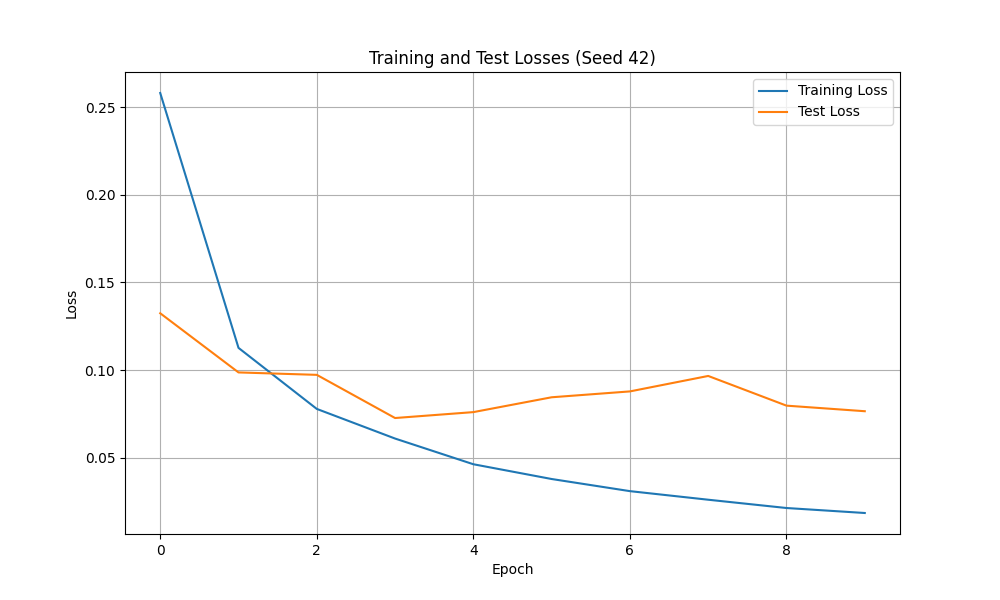
\includegraphics[width=0.7\textwidth]{loss_curves.png}
    \caption{Training and test error curves during training for Task 1.}
    \label{fig:task1_curves}
\end{figure}

The final test error achieved was [insert your test error here].

\subsection{Misclassified Examples}

% Insert your misclassified images plot here
\begin{figure}[H]
    \centering
    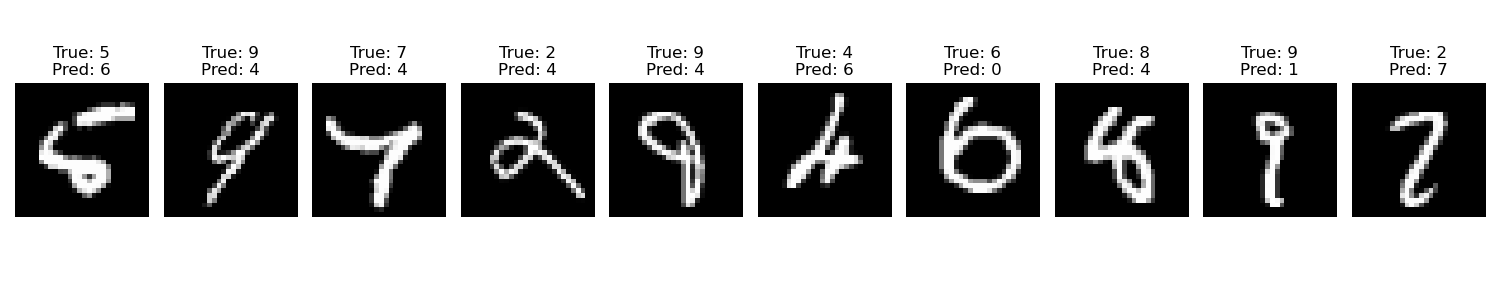
\includegraphics[width=0.9\textwidth]{misclassified_images.png}
    \caption{Examples of misclassified digits. The true label is shown above each image, and the model's prediction is shown below.}
    \label{fig:misclassified}
\end{figure}

Analysis of misclassified examples:
[Write a brief analysis of the types of errors the model makes and any patterns observed]

\section{Task 2: Mitigating Pseudorandomness}

In this task, we adapted our code to ensure reproducibility by setting seeds for all random number generators. We then ran the model with 5 different seed values to analyze the variability in results.

\subsection{Implementation Approach}
To mitigate pseudorandomness, we implemented the following approach:
\begin{itemize}
    \item Set seeds for all sources of randomness in PyTorch, NumPy, and Python's random module
    \item Set CuDNN to deterministic mode
    \item Fixed the environmental seed
    \item Trained the model with 5 different seeds: [list your seeds]
\end{itemize}

\subsection{Results}

% Insert your test error curves for different seeds plot here
\begin{figure}[H]
    \centering
    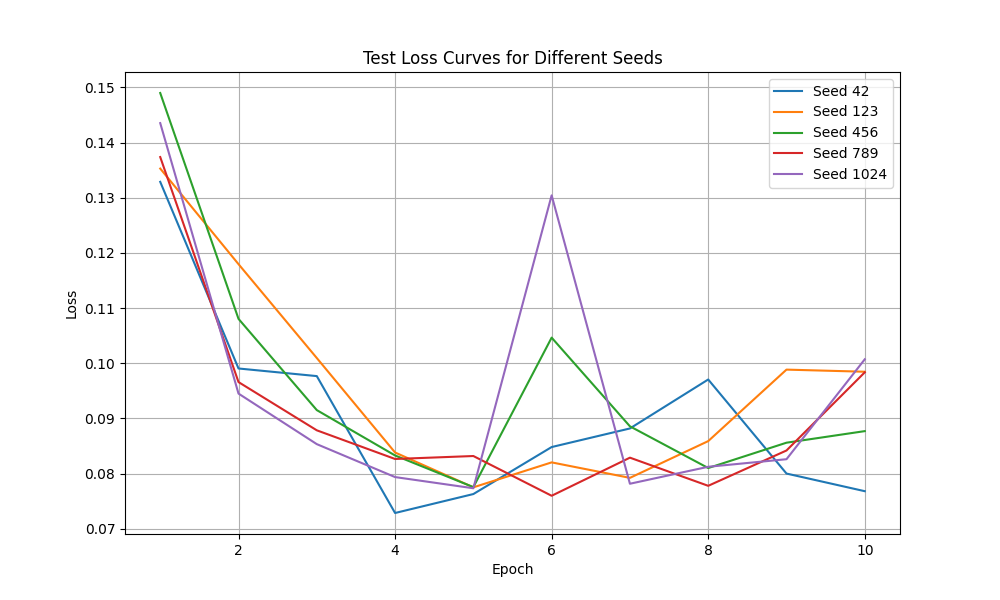
\includegraphics[width=0.7\textwidth]{seed_test_loss_curves.png}
    \caption{Test error curves for models trained with different seeds.}
    \label{fig:seed_curves}
\end{figure}

\begin{table}[H]
    \centering
    \caption{Final Test Errors for Different Seeds}
    \label{tab:seed_results}
    \begin{tabular}{ccc}
        \toprule
        Seed & Test Loss & Test Accuracy (\%) \\
        \midrule
        [Seed 1] & [Loss 1] & [Acc 1] \\
        [Seed 2] & [Loss 2] & [Acc 2] \\
        [Seed 3] & [Loss 3] & [Acc 3] \\
        [Seed 4] & [Loss 4] & [Acc 4] \\
        [Seed 5] & [Loss 5] & [Acc 5] \\
        \midrule
        Mean & [Mean Loss] & [Mean Acc] \\
        Std Dev & [Std Loss] & [Std Acc] \\
        \bottomrule
    \end{tabular}
\end{table}

\subsection{Analysis}
Based on the standard deviation of test errors ([insert std dev value]), we can conclude that our model is [insert robustness conclusion: highly robust/robust/moderately robust/not robust] to the choice of seed number. 

[Add additional analysis about the observed variance and what it indicates about model training]

\section{Task 3: Validation Dataset}

In this task, we split the MNIST dataset into three sets: training, validation, and test. We then trained models with 5 different seeds and reported the test error corresponding to the minimum validation error obtained during training.

\subsection{Implementation Details}
Our implementation includes:
\begin{itemize}
    \item Splitting the original training set into training and validation sets (10,000 images for validation)
    \item Training models with 5 different seeds
    \item Monitoring both validation and test errors after each epoch
    \item Reporting the test error corresponding to the epoch with minimum validation error
\end{itemize}

\subsection{Results}

\begin{table}[H]
    \centering
    \caption{Best Validation Errors and Corresponding Test Errors}
    \label{tab:val_results}
    \begin{tabular}{ccc}
        \toprule
        Seed & Best Validation Loss & Corresponding Test Loss \\
        \midrule
        [Seed 1] & [Val Loss 1] & [Test Loss 1] \\
        [Seed 2] & [Val Loss 2] & [Test Loss 2] \\
        [Seed 3] & [Val Loss 3] & [Test Loss 3] \\
        [Seed 4] & [Val Loss 4] & [Test Loss 4] \\
        [Seed 5] & [Val Loss 5] & [Test Loss 5] \\
        \midrule
        Mean & [Mean Val] & [Mean Test] \\
        Std Dev & [Std Val] & [Std Test] \\
        \bottomrule
    \end{tabular}
\end{table}

% Insert your validation vs test error comparison plot here
\begin{figure}[H]
    \centering
    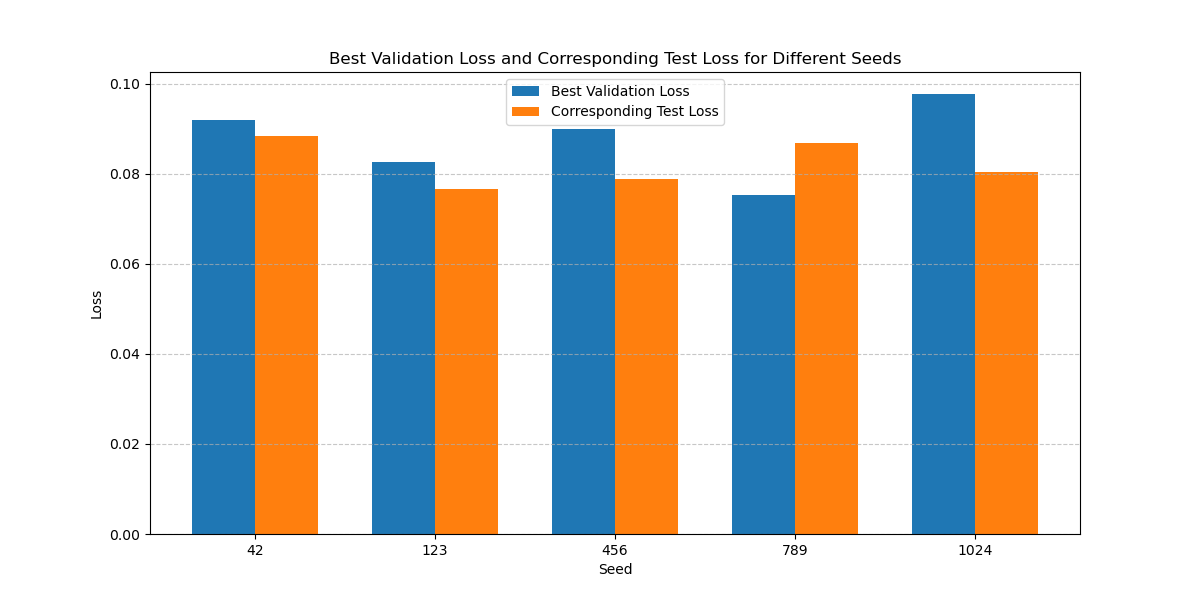
\includegraphics[width=0.7\textwidth]{validation_test_loss_comparison.png}
    \caption{Comparison of best validation losses and corresponding test losses for different seeds.}
    \label{fig:val_test_comparison}
\end{figure}

\subsection{Analysis}
[Analyze the relationship between validation and test errors, and discuss how validation helps in model selection]

\section{Task 4: Grid Search}

In this task, we performed a grid search over three hyperparameters: hidden layer size, batch size, and learning rate. We trained models for each combination of parameters and reported the test error corresponding to the best validation error for every combination.

\subsection{Implementation Details}
Our grid search explored the following parameter values:
\begin{itemize}
    \item Hidden sizes: [list your values]
    \item Batch sizes: [list your values]
    \item Learning rates: [list your values]
\end{itemize}

This resulted in [X] models being trained and evaluated.

\subsection{Results}

% Insert your grid search results table here
% You can use the CSV file generated or create a table directly
\begin{table}[H]
    \centering
    \caption{Grid Search Results (Sorted by Validation Loss)}
    \label{tab:grid_search}
    \begin{tabular}{cccccc}
        \toprule
        Hidden Size & Batch Size & Learning Rate & Validation Loss & Test Loss & Test Accuracy (\%) \\
        \midrule
        [Value] & [Value] & [Value] & [Value] & [Value] & [Value] \\
        [Value] & [Value] & [Value] & [Value] & [Value] & [Value] \\
        % ... more rows
        \bottomrule
    \end{tabular}
\end{table}

% Insert your heatmap visualization here
\begin{figure}[H]
    \centering
    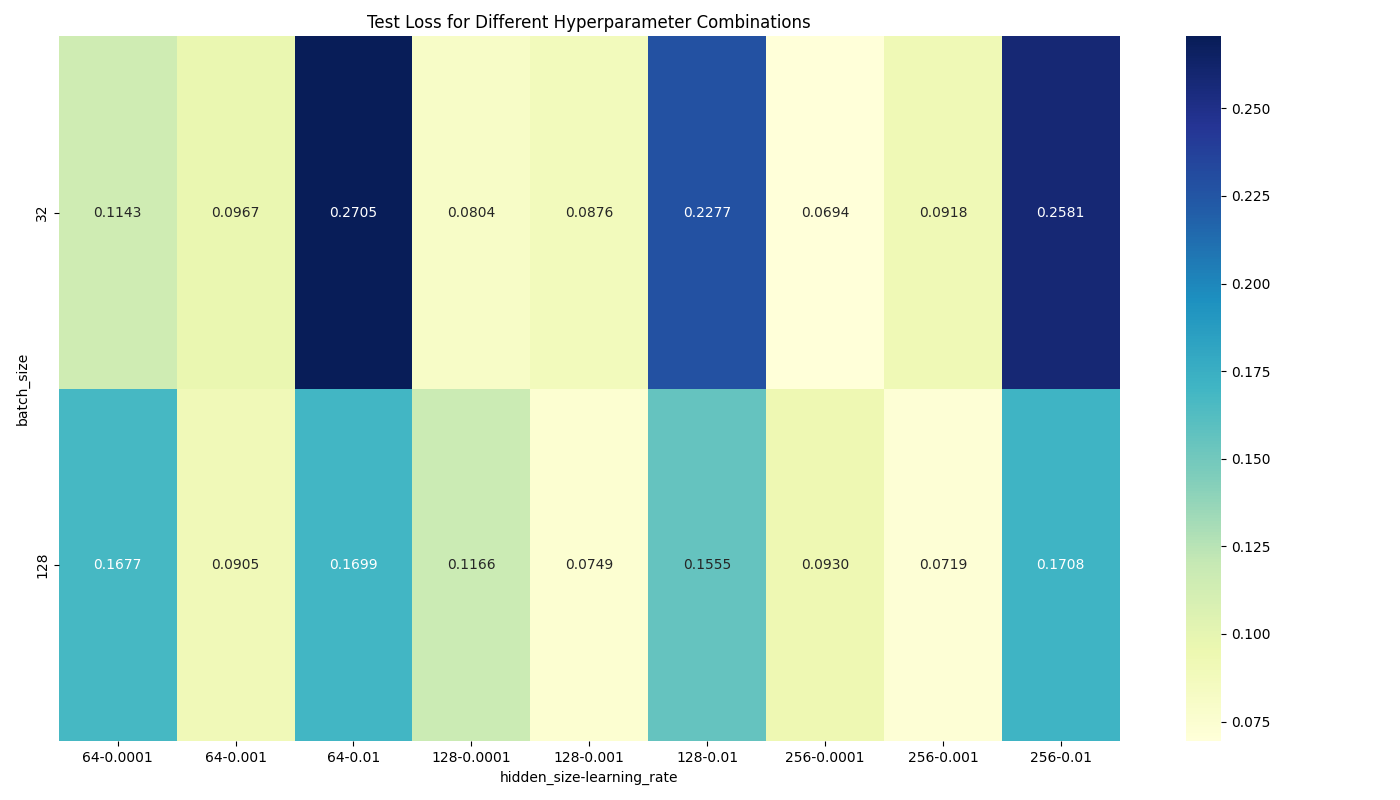
\includegraphics[width=0.8\textwidth]{grid_search_heatmap.png}
    \caption{Heatmap of test loss for different hyperparameter combinations.}
    \label{fig:heatmap}
\end{figure}

\subsection{Analysis}
The best combination of hyperparameters was:
\begin{itemize}
    \item Hidden size: [best value]
    \item Batch size: [best value]
    \item Learning rate: [best value]
\end{itemize}

This combination achieved a validation loss of [value] and a test loss of [value].

[Add analysis of trends observed across different hyperparameters and insights gained from the grid search]

\section{Task 5: Feature Analysis}

In this task, we visualized and analyzed the hidden features of the neural network using t-SNE dimensionality reduction. We compared the t-SNE visualizations of the input features and hidden features to understand what the network has learned.

\subsection{Implementation Details}
For this analysis, we:
\begin{itemize}
    \item Trained a model with the best hyperparameters from Task 4
    \item Extracted both input features (flattened images) and hidden features (activations from the hidden layer)
    \item Applied t-SNE to reduce both feature sets to 2 dimensions
    \item Created visualizations with color-coding based on digit class
\end{itemize}

\subsection{Results}

% Insert your t-SNE visualizations here
\begin{figure}[H]
    \centering
    \begin{subfigure}{0.48\textwidth}
        \includegraphics[width=\textwidth]{task5_tsne_input_features.png}
        \caption{t-SNE of Input Features}
    \end{subfigure}
    \hfill
    \begin{subfigure}{0.48\textwidth}
        \includegraphics[width=\textwidth]{task5_tsne_hidden_features.png}
        \caption{t-SNE of Hidden Features}
    \end{subfigure}
    \caption{t-SNE visualizations of input and hidden features.}
    \label{fig:tsne}
\end{figure}

\subsection{Analysis}
[Analyze the differences between the input and hidden feature visualizations. Discuss what these differences tell us about what the model has learned. Comment on cluster formations, separations between digits, and any interesting patterns observed.]

Key observations include:
\begin{itemize}
    \item [Observation 1]
    \item [Observation 2]
    \item [Observation 3]
    \item [Observation 4]
\end{itemize}

These observations indicate that the neural network has learned to [describe what the network has learned based on the visualizations].

\section{Conclusion}

In this assignment, we implemented and experimented with feedforward neural networks for MNIST digit classification. Our key findings include:

\begin{itemize}
    \item [Key finding from Task 1]
    \item [Key finding from Task 2]
    \item [Key finding from Task 3]
    \item [Key finding from Task 4]
    \item [Key finding from Task 5]
\end{itemize}

These experiments have demonstrated [summarize overall insights about neural network behavior, hyperparameter selection, and feature learning].

\end{document}
